% -*- TeX-engine: xetex; eval: (auto-fill-mode 0); eval: (visual-line-mode 1); -*-
% Compile with XeLaTeX

%%%%%%%%%%%%%%%%%%%%%%%
% To do before class
%%%%%%%%%%%%%%%%%%%%%%%

% Send the Logistics/Week0Annoucnement (the night before).
% Send an email reminding students to bring a charged computer (the night before).

%%%%%%%%%%%%%%%%%%%%%%%
% Option 1: Slides: (comment for handouts)   %
%%%%%%%%%%%%%%%%%%%%%%%

\documentclass[slidestop,compress,mathserif,12pt,t,professionalfonts,xcolor=table]{beamer}

% solution stuff
\newcommand{\solnMult}[1]{
\only<1>{#1}
\only<2->{\red{\textbf{#1}}}
}
\newcommand{\soln}[1]{\textit{#1}}

\newcommand{\solnMultOn}[3]{
\only<#1>{#3}
\only<{#2}->{\red{\textbf{#3}}}
}

%%%%%%%%%%%%%%%%%%%%%%%%%%%%%%%
% Option 2: Handouts, without solutions (post before class)    %
%%%%%%%%%%%%%%%%%%%%%%%%%%%%%%%

% \documentclass[11pt,containsverbatim,handout,xcolor=xelatex,dvipsnames,table]{beamer}

% % handout layout
% \usepackage{pgfpages}
% \pgfpagesuselayout{4 on 1}[letterpaper,landscape,border shrink=5mm]

% % solution stuff
% \newcommand{\solnMult}[1]{#1}
% \newcommand{\soln}[1]{}
% \newcommand{\solnMultOn}[3]{#3}

% % % This breaks things for me for some reason.
% % tell pgfpages how to set page sizes in XeLaTeX
% %\renewcommand\pgfsetupphysicalpagesizes{%
% %   \pdfpagewidth\pgfphysicalwidth\pdfpageheight\pgfphysicalheight%
% %}

%%%%%%%%%%%%%%%%%%%%%%%%%%%%%%%%%%%%
% Option 3: Handouts, with solutions (may post after class if need be)    %
%%%%%%%%%%%%%%%%%%%%%%%%%%%%%%%%%%%%

% \documentclass[11pt,containsverbatim,handout,xcolor=xelatex,dvipsnames,table]{beamer}

% % handout layout
% \usepackage{pgfpages}
% \pgfpagesuselayout{4 on 1}[letterpaper,landscape,border shrink=5mm]

% % solution stuff
% \newcommand{\solnMult}[1]{\red{\textbf{#1}}}
% \newcommand{\soln}[1]{\textit{#1}}

% % % This breaks things for me for some reason.
% % % tell pgfpages how to set page sizes in XeLaTeX
% % \renewcommand\pgfsetupphysicalpagesizes{%
% %    \pdfpagewidth\pgfphysicalwidth\pdfpageheight\pgfphysicalheight%
% % }

%%%%%%%%%%%%%%%%%%%%%%%%%%%%%%%
% Option 4: Notes Only
%%%%%%%%%%%%%%%%%%%%%%%%%%%%%%%

% % See http://tex.stackexchange.com/questions/114219/add-notes-to-latex-beamer
% \documentclass[10pt,containsverbatim,xcolor=xelatex,dvipsnames,table,notes=only]{beamer}

% % handout layout
% % \usepackage{pgfpages}
% % \pgfpagesuselayout{1 on 1}[letterpaper, landscape, border shrink=5mm]

% % solution stuff
% \newcommand{\solnMult}[1]{#1}
% \newcommand{\soln}[1]{}

% % % Having a problem with this.
% % tell pgfpages how to set page sizes in XeLaTeX
% % \renewcommand\pgfsetupphysicalpagesizes{%
% %   \pdfpagewidth\pgfphysicalwidth\pdfpageheight\pgfphysicalheight%
% %}

%%%%%%%%%%
% Load style file, defaults  %
%%%%%%%%%%

\input{../../lec_style.tex}
% You cannot use numbers when defining variables.  Hence the use of letters, A, B, C, etc.

% Personal Info
\newcommand{\FirstName}{Mine}
\newcommand{\LastName}{\c{C}etinkaya-Rundel}
\newcommand{\OfficeHours}{MTWR 3-4pm.}
\newcommand{\OfficeHoursLocation}{Old Chem 213}

% Electronic Info
\newcommand{\PersonalSite}{http://stat.duke.edu/~mc301}
\newcommand{\CourseSite}{http://bitly.com/sta101sp15}
\newcommand{\Email}{mine@stat.duke.edu}

% TAs
\newcommand{\TAA}{Anthony Weishampel}
\newcommand{\TAB}{Fiamma Li}
\newcommand{\TAC}{Jialiang Mao}
\newcommand{\TAD}{Phillip Lee}

% Exam Dates
\newcommand{\ExamADate}{Wed, Feb 18}
\newcommand{\ExamBDate}{Wed, Mar 25}
\newcommand{\FinalDate}{Sat, May 2 (2-5pm)}

% Due Dates
\newcommand{\ClickerRegistrationDD}{Mon, Jan 26}
\newcommand{\GettingToKnowYouDD}{Friday, Jan 9, 11:59pm}
\newcommand{\ProblemSetADD}{Wed., 1/15}


% ALT ALT
%% You cannot use numbers when defining variables.  Hence the use of letters, A, B, C, etc.

% Personal Info
\renewcommand{\FirstName}{Jesse}
\renewcommand{\LastName}{Windle}
\renewcommand{\OfficeHours}{Tue, Thu 3:00pm-4:30pm}
\renewcommand{\OfficeHoursLocation}{Old Chem 211D}

% Electronic Info
\renewcommand{\PersonalSite}{http://stat.duke.edu/~jbw44/}
\renewcommand{\CourseSite}{http://bitly.com/windle2}
\renewcommand{\Email}{jbw44@stat.duke.edu}

% TAs
\renewcommand{\TAA}{David Clancy}
\renewcommand{\TAB}{Xinyi (Chris) Li}
\renewcommand{\TAC}{Tori Hall}
\renewcommand{\TAD}{Radhika Anand}

% Exam Dates
\renewcommand{\ExamADate}{Thu, Feb 19}
\renewcommand{\ExamBDate}{Thu, Mar 26}
\renewcommand{\FinalDate}{Mon, Apr 27 (9-Noon)}

% Due Dates
\renewcommand{\ClickerRegistrationDD}{Thu, Jan 15}
\renewcommand{\GettingToKnowYouDD}{Friday, Jan 9, 11:59pm}
\renewcommand{\ProblemSetADD}{Thu., 1/16}

%%%%%%%%%%%
% Cover slide info    %
%%%%%%%%%%%

\title{Unit 7: Multiple linear regression}
\subtitle{3. Confidence and prediction intervals \& transformations}
\author{Sta 101 - Spring 2015}
\date{April 13, 2015}
\institute{Duke University, Department of Statistical Science}

%%%%%%%%%%%
% Begin document   %
%%%%%%%%%%%

\begin{document}

%%%%%%%%%%%%%%%%%%%%%%%%%%%%%%%%%%%%

% Title Page

\begin{frame}[plain]

\titlepage
\vfill
{\scriptsize \webLink{\PersonalSite}{Dr. \LastName{}} \hfill Slides posted at  \webLink{\CourseSite}{\CourseSite}}
\addtocounter{framenumber}{-1} 

\end{frame}

%%%%%%%%%%%%%%%%%%%%%%%%%%%%%%%%%%%%

\section{Housekeeping}

%%%%%%%%%%%%%%%%%%%%%%%%%%%%%%%%%%%%

\begin{frame}
\frametitle{Announcements}

\begin{itemize}

\item 

\end{itemize}

\end{frame}

%%%%%%%%%%%%%%%%%%%%%%%%%%%%%%%%%%%

\section{Uncertainty of predictions}

%%%%%%%%%%%%%%%%%%%%%%%%%%%%%%%%%%%%

\begin{frame}
\frametitle{Uncertainty of predictions}

\begin{itemize}

\item Regression models are useful for making predictions for new observations not include in the original dataset.

\pause

\item If the model is good, the predictions should be close to the true value of the response variable for this observation, however it may not be exact, i.e. $\hat{y}$ might be different than $y$.

\pause

\item With any prediction we can (and should) also report a measure of uncertainty of the prediction:
\begin{itemize}
\item Use a \hl{confidence interval} for the uncertainty around the expected value of predictions (average of a group of predictions) -- e.g. predict the average final exam score of a group of students who scored the same on the midterm.
\item Use a \hl{prediction interval} for the uncertainty around a single prediction -- e.g. predict the final exam score of one student with a given midterm score.
\end{itemize}

\end{itemize}

\end{frame}

%%%%%%%%%%%%%%%%%%%%%%%%%%%%%%%%%%%%

\subsection{Confidence intervals for average values}

%%%%%%%%%%%%%%%%%%%%%%%%%%%%%%%%%%%%

\begin{frame}
\frametitle{}

\formula{Confidence intervals for average values}{
A confidence interval for the average (expected) value of $y$, $E(y)$, for a given $x^\star$, is
\[ \hat{y} \pm t^\star_{n - 2} s \sqrt{ \frac{1}{n} + \frac{(x^\star - \bar{x})^2}{(n - 1)s_x^2} } \]
where $s$ is the standard deviation of the residuals, calculated as $\sqrt{\frac{\sum(y_i - \hat{y}_i)^2}{n-2}}$.
}

\end{frame}

%%%%%%%%%%%%%%%%%%%%%%%%%%%%%%%%%%%

\begin{frame}[fragile]
\frametitle{}

\disc{Calculate a 95\% confidence interval for the average IQ score of foster twins whose biological twins have IQ scores of 100 points. Note that the average IQ score of 27 biological twins in the sample is 95.3 points, with a standard deviation is 15.74 points.}
 
{\scriptsize
\begin{verbatim}
                 Estimate Std. Error t value Pr(>|t|)    
(Intercept)       9.20760    9.29990   0.990    0.332    
bioIQ             0.90144    0.09633   9.358  1.2e-09

Residual standard error: 7.729 on 25 degrees of freedom
\end{verbatim}
}

\twocol{0.4}{0.65}
{
\only<1|handout:0>{\includegraphics[width=\textwidth]{figures/twins/twins_IQ}}
\only<2-7|handout:0>{\includegraphics[width=\textwidth]{figures/twins/twins_IQ_100pred}}
\only<8>{\includegraphics[width=\textwidth]{figures/twins/twins_IQ_100cint}}
}
{
\pause
{\small
\begin{eqnarray*}
\hat{y} &=& 9.2076 + 0.90144 \times 100 \approx 99.35 \\ \pause
df &=& n-2 \pause\qquad t^\star = 2.06 \\ \pause
ME &=& 2.06 \times 7.729 \times \sqrt{\frac{1}{27} + \frac{(100 - 95.3)^2}{26 \times 15.74^2}} \\ \pause
&\approx& 3.2 \\ \pause
CI &=& 99.35 \pm 3.2 \\ \pause
&=& (96.15, 102.55)
\end{eqnarray*}
}
}

\end{frame}

%%%%%%%%%%%%%%%%%%%%%%%%%%%%%%%%%%%

\begin{frame}[fragile]
\frametitle{Confidence interval for a prediction -- in R}

{\footnotesize
\begin{Verbatim}[frame=single, formatcom=\color{blue}]
# load data
install.packages("faraway") # dataset is in this package
library(faraway)
data(twins)

# fit model
m = lm(Foster ~ Biological, data = twins)

# create a new data frame for the new observation
newdata = data.frame(Biological = 100)

# calculate a prediction 
# and a confidence interval for the prediction
predict(m , newdata, interval = "confidence")
\end{Verbatim}
}

\pause

{\footnotesize
\begin{Verbatim}[frame=single, formatcom=\color{gray}]
     fit      lwr      upr
 99.3512 96.14866 102.5537
\end{Verbatim}
}

\end{frame}

%%%%%%%%%%%%%%%%%%%%%%%%%%%%%%%%%%%

\begin{frame}

\clicker{How would you expect the width of the 95\% confidence interval for the average IQ score of foster twins whose biological twins have IQ scores of 130 points ($x^\star = 130$) to compare to the previous confidence interval (where $x^\star = 100$)?}

\twocol{0.5}{0.5}
{
\includegraphics[width=\textwidth]{figures/twins/twins_IQ_100cint_130pred}
}
{
\begin{enumerate}[(a)]
\item \solnMult{wider}
\item narrower
\item same width
\item cannot tell
\end{enumerate}
}

\end{frame}


%%%%%%%%%%%%%%%%%%%%%%%%%%%%%%%%%%%

\begin{frame}[fragile]
\frametitle{}

\disc{How do the confidence intervals where $x^\star = 100$ and $x^\star = 130$ compare in terms of their widths?}
 
\twocol{0.2}{0.8}
{
\onslide<1->{\[ x^\star = 100 \]}
\onslide<2->{\[ x^\star = 130 \]}
}
{
\onslide<1->{\[ ME_{100} = 2.06 \times 7.729 \times \sqrt{\frac{1}{27} + \frac{(\red{100} - 95.3)^2}{26 \times 15.74^2}} = 3.2\]}
\onslide<3->{\[ ME_{130} = 2.06 \times 7.729 \times \sqrt{\frac{1}{27} + \frac{(\red{130} - 95.3)^2}{26 \times 15.74^2}} =}\onslide<4->{ 7.53 \]}
}

\onslide<5->{
\begin{center}
\includegraphics[width=0.5\textwidth]{figures/twins/twins_IQ_100cint_130cint}
\end{center}
}

\end{frame}


%%%%%%%%%%%%%%%%%%%%%%%%%%%%%%%%%%%

\begin{frame}
\frametitle{Recap}

\vspace{-0.25cm}

The width of the confidence interval for $E(y)$ increases as $x^\star$ moves away from the center.

\begin{itemize}

\item Conceptually: We are much more certain of our predictions at the center of the data than at the edges (and our level of certainty decreases even further when predicting outside the range of the data -- extrapolation).

\item Mathematically: As $(x^\star - \bar{x})^2$ term increases, the margin of error of the confidence interval increases as well.

\end{itemize}

\begin{center}
\includegraphics[width=0.5\textwidth]{figures/twins/twins_IQ_cint}
\end{center}

\end{frame}

%%%%%%%%%%%%%%%%%%%%%%%%%%%%%%%%%%%

\subsection{Prediction intervals for specific predicted values}

%%%%%%%%%%%%%%%%%%%%%%%%%%%%%%%%%%%%

\begin{frame}
\frametitle{}

\clicker{Earlier we learned how to calculate a confidence interval for average $y$, $E(y)$, for a given $x^\star$. \\

Suppose we're not interested in the average, but instead we want to predict a future value of $y$ for a given $x^\star$. \\

Would you expect there to be more uncertainty around an average or a specific predicted value?}

\begin{enumerate}[(a)]
\item more uncertainty around an average
\item \solnMult{more uncertainty around a specific predicted value}
\item equal uncertainty around both values
\item cannot tell
\end{enumerate}

\end{frame}

%%%%%%%%%%%%%%%%%%%%%%%%%%%%%%%%%%%%

\begin{frame}
\frametitle{}

\formula{Prediction intervals for specific predicted values}{
A \hl{prediction interval} for $y$ for a given $x^\star$ is
\[ \hat{y} \pm t^\star_{n - 2} s \sqrt{ 1 + \frac{1}{n} + \frac{(x^\star - \bar{x})^2}{(n - 1)s_x^2} } \]
where $s$ is the standard deviation of the residuals.
}

\pause

\begin{itemize}

\item The formula is very similar, except the variability is higher since there is an added 1 in the formula.

\pause

\item Prediction level: If we repeat the study of obtaining a regression data set many times, each time forming a XX\% prediction interval at $x^\star$, and wait to see what the future value of $y$ is at $x^\star$, then roughly XX\% of the prediction intervals will contain the corresponding actual value of $y$.

\end{itemize}

\end{frame}

%%%%%%%%%%%%%%%%%%%%%%%%%%%%%%%%%%%

\begin{frame}[fragile]
\frametitle{}

\vfill

\app{7.3 Prediction interval}{See course website for details}

\vfill

\soln{
\pause
We already found that $\hat{y} \approx 99.35$ and $t_{25}^\star = 2.06$. 
\begin{eqnarray*}
ME &=& 2.06 \times 7.729 \times \sqrt{1 + \frac{1}{27} + \frac{(100 - 95.3)^2}{26 \times 15.74^2}} \approx 16.24 \\ \pause
CI &=& 99.35 \pm 16.24 \\ \pause
&=& (83.11, 115.59)
\end{eqnarray*}
}

\end{frame}

%%%%%%%%%%%%%%%%%%%%%%%%%%%%%%%%%%%

\subsection{Recap - CI vs. PI}

%%%%%%%%%%%%%%%%%%%%%%%%%%%%%%%%%%%

\begin{frame}
\frametitle{CI for $E(y)$ vs. PI for $y$ (1)}

\begin{center}
\includegraphics[width=\textwidth]{figures/twins/twins_IQ_100cintpint_130cintpint}
\end{center}

\end{frame}

%%%%%%%%%%%%%%%%%%%%%%%%%%%%%%%%%%%

\begin{frame}
\frametitle{CI for $E(y)$ vs. PI for $y$ (2)}

\begin{center}
\includegraphics[width=\textwidth]{figures/twins/twins_IQ_cint_pint}
\end{center}

\end{frame}

%%%%%%%%%%%%%%%%%%%%%%%%%%%%%%%%%%%


\begin{frame}
\frametitle{CI for $E(y)$ vs. PI for $y$ - differences}

\begin{itemize}

\item A prediction interval is similar in spirit to a confidence interval, except that 
\pause
\begin{itemize}
\item the prediction interval is designed to cover a ``moving target", \\
the random future value of $y$, while
\pause
\item the confidence interval is designed to cover the ``fixed target", \\
the average (expected) value of $y$, $E(y)$,
\end{itemize}
for a given $x^\star$.

\pause

\item Although both are centered at $\hat{y}$, the prediction interval is wider than the confidence interval, for a given $x^\star$ and confidence level. This makes sense, since
\pause
\begin{itemize}
\item the prediction interval must take account of the tendency of $y$ to fluctuate from its mean value, while 
\pause
\item the confidence interval simply needs to account for the uncertainty in estimating the mean value.
\end{itemize}

\end{itemize}

\end{frame}

%%%%%%%%%%%%%%%%%%%%%%%%%%%%%%%%%%%

\begin{frame}
\frametitle{CI for $E(y)$ vs. PI for $y$ - similarities}

\begin{itemize}

\item For a given data set, the error in estimating $E(y)$ and $\hat{y}$ grows as $x^\star$ moves away from $\bar{x}$. Thus, the further $x^\star$ is from $\bar{x}$, the wider the confidence and prediction intervals will be.

\pause

\item If any of the conditions underlying the model are violated, then the confidence intervals and prediction intervals may be invalid as well. This is why it's so important to check the conditions by examining the residuals, etc.

\end{itemize}

\end{frame}

%%%%%%%%%%%%%%%%%%%%%%%%%%%%%%%%%%%

\subsection{Confidence and prediction intervals for MLR}

%%%%%%%%%%%%%%%%%%%%%%%%%%%%%%%%%%%

\begin{frame}
\frametitle{Confidence and prediction intervals for MLR}

\begin{itemize}

\item In the case of multiple linear regression (regression with many predictors), confidence and prediction intervals for a new prediction works exactly the same way.

\item However the formulas are much more complicated since we no longer have just one $x$, but instead many $x$s.

\item For confidence and prediction intervals for MLR we will focus on the concepts and leave the calculations up to R.

\end{itemize}

\end{frame}

%%%%%%%%%%%%%%%%%%%%%%%%%%%%%%%%%%%

\begin{frame}[fragile]
\frametitle{Prediction of evaluation my evaluation score}

\vspace{-0.2cm}

{\footnotesize
\begin{Verbatim}[frame=single, formatcom=\color{blue}]
# fit a model
m = lm(score ~ rank + gender + language + 
    cls_perc_eval + cls_students, data = evals)

# create a data frame with the new observation (mine)
prof = data.frame(rank = "teaching", gender = "female", 
    language = "english", cls_perc_eval = 90, 
    cls_students = 100)
\end{Verbatim}
}

\pause

{\footnotesize
\begin{Verbatim}[frame=single, formatcom=\color{blue}]
predict(m , prof , interval = "prediction")
\end{Verbatim}
}

\pause

{\footnotesize
\begin{Verbatim}[frame=single, formatcom=\color{gray}]
      fit     lwr      upr
 4.337951 3.301877 5.374026
\end{Verbatim}
}

\pause

{\footnotesize
\begin{Verbatim}[frame=single, formatcom=\color{blue}]
predict(m , prof , interval = "confidence")
\end{Verbatim}
}

\pause

{\footnotesize
\begin{Verbatim}[frame=single, formatcom=\color{gray}]
      fit     lwr      upr
 4.337951 4.20273 4.473172
\end{Verbatim}
}

\end{frame}

%%%%%%%%%%%%%%%%%%%%%%%%%%%%%%%%%%%

\section{Transformations}

%%%%%%%%%%%%%%%%%%%%%%%%%%%%%%%%%%%%

\begin{frame}[fragile]
\frametitle{Truck prices}

\disc{The scatterplot below shows the relationship between year and price of a random sample of 43 pickup trucks. Describe the relationship between these two variables.}

\begin{center}
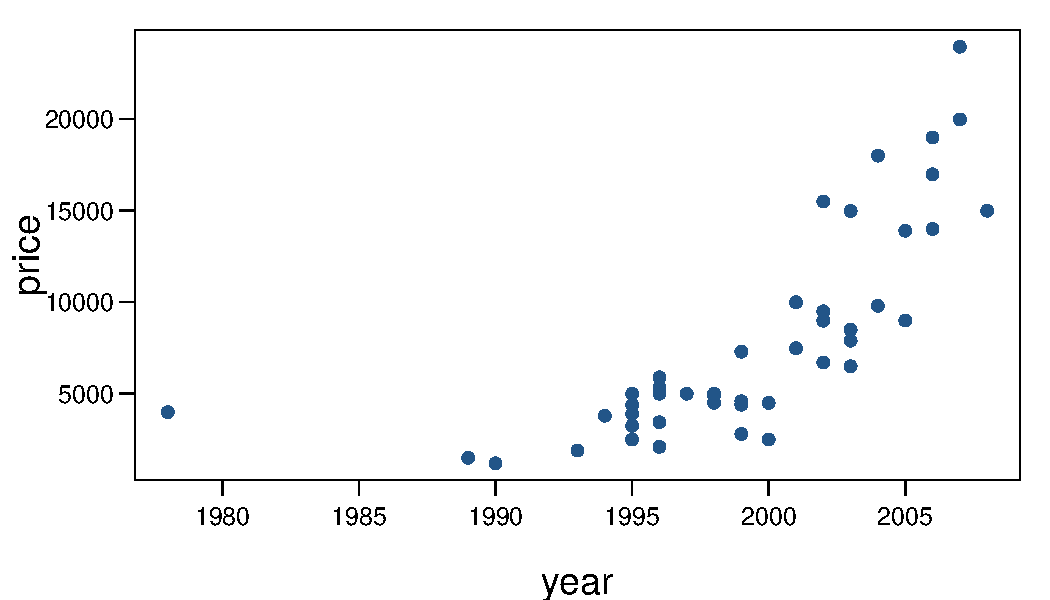
\includegraphics[width=0.7\textwidth]{figures/pickup/pu_price_year_scat_allyrs}
\end{center}

\ct{From: \webURL{http://faculty.chicagobooth.edu/robert.gramacy/teaching.html}}


\end{frame}

%%%%%%%%%%%%%%%%%%%%%%%%%%%%%%%%%%%

\begin{frame}[fragile]
\frametitle{Remove unusual observations}

Let's remove trucks older than 20 years, and only focus on trucks made in 1992 or later.

\pause

\disc{Now what can you say about the relationship?}

\begin{center}
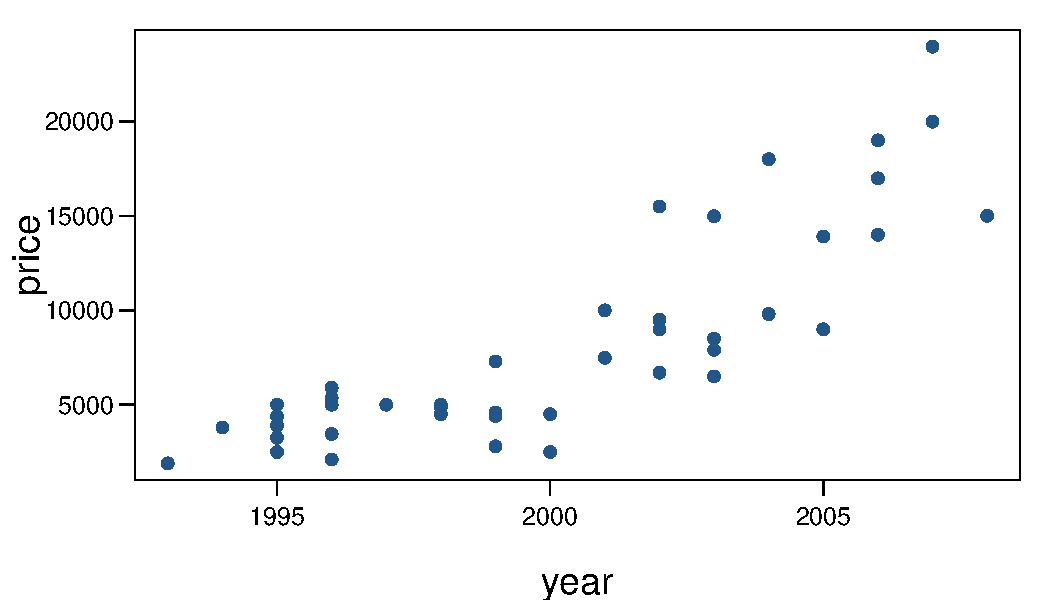
\includegraphics[width=0.7\textwidth]{figures/pickup/pu_price_year_scat_noline}
\end{center}

\end{frame}

%%%%%%%%%%%%%%%%%%%%%%%%%%%%%%%%%%%

\begin{frame}
\frametitle{Truck prices - linear model?}

\vspace{-0.25cm}

\twocol{0.63}{0.35}
{
\begin{center}
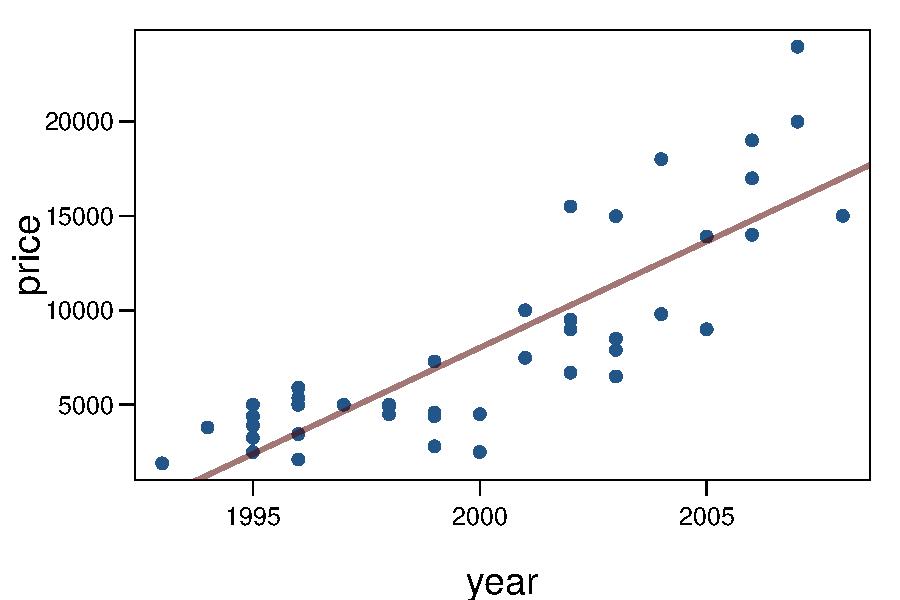
\includegraphics[width=\textwidth]{figures/pickup/pu_price_year_scat} \\
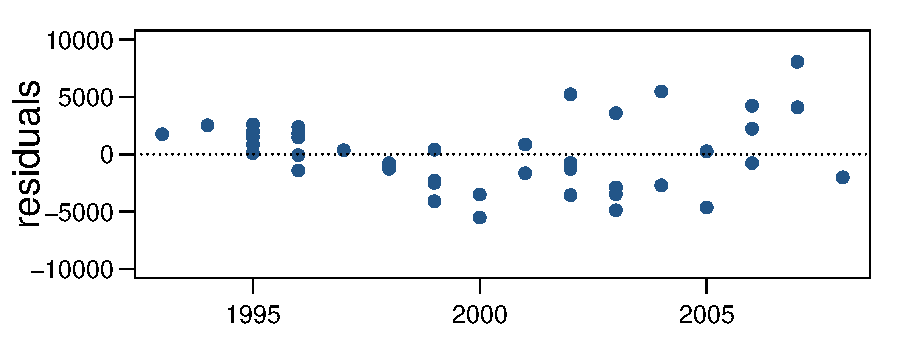
\includegraphics[width=\textwidth]{figures/pickup/pu_price_year_res}
\end{center}
}
{
\hl{Model:} \[ \widehat{price} = b_0 + b_1~year \]
\pause
The linear model doesn't appear to be a good fit since the residuals have non-constant variance. \\
}

\end{frame}

%%%%%%%%%%%%%%%%%%%%%%%%%%%%%%%%%%%

\begin{frame}
\frametitle{Truck prices - log transform of the response variable}

\vspace{-0.25cm}

\twocol{0.63}{0.35}
{
\begin{center}
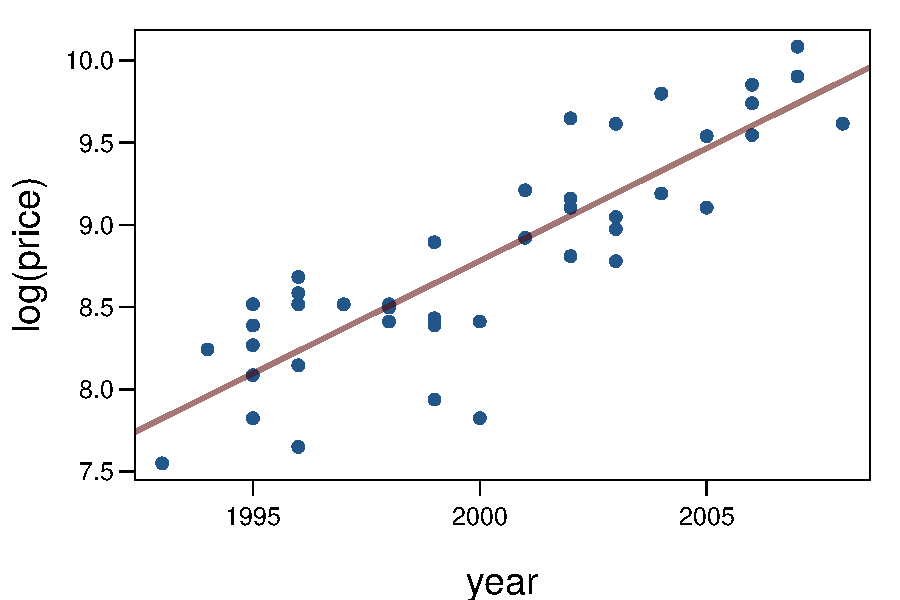
\includegraphics[width=\textwidth]{figures/pickup/pu_price_year_scat_log} \\
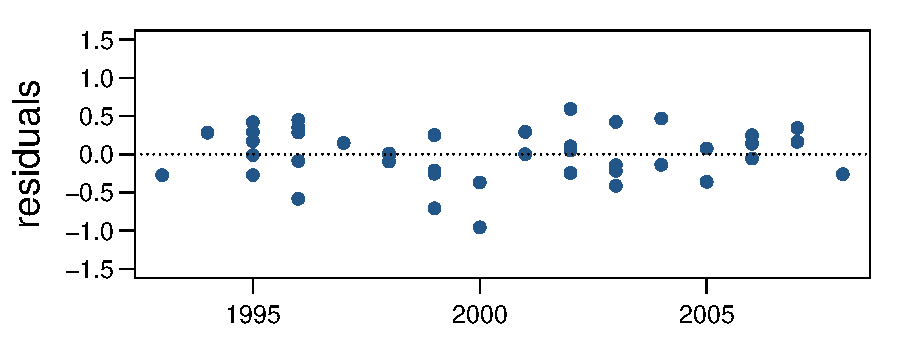
\includegraphics[width=\textwidth]{figures/pickup/pu_price_year_res_log}
\end{center}
}
{
\hl{Model:} \[ \widehat{log(price)} = b_0 + b_1~year \]
\pause
We applied a log transformation to the response variable. The relationship now seems linear, and the residuals no longer have non-constant variance.
}

\end{frame}

%%%%%%%%%%%%%%%%%%%%%%%%%%%%%%%%%%%

\begin{frame}
\frametitle{Interpreting models with log transformation}

\begin{center}
\begin{tabular}{rrrrr}
  \hline
 & Estimate & Std. Error & t value & Pr($>$$|$t$|$) \\ 
  \hline
(Intercept) & -265.07 & 25.04 & -10.59 & 0.00 \\ 
  pu\$year & 0.14 & 0.01 & 10.94 & 0.00 \\ 
   \hline
\end{tabular}
\end{center}

\pause
\[ \hl{\text{Model: }} \widehat{log(price)} = -265.07 + 0.14~year \]

\pause

\begin{itemize}

\item For each additional year the car is newer (for each year decrease in car's age) we would expect the log price of the car to increase on average by 0.14 log dollars.

\pause

\item which is not very useful...

\end{itemize}

\end{frame}

%%%%%%%%%%%%%%%%%%%%%%%%%%%%%%%%%%%

\begin{frame}
\frametitle{Working with logs}

\begin{itemize}

\item Subtraction and logs: $log(a) - log(b) = log(\frac{a}{b})$

\pause

\item Natural logarithm: $e^{log(x)} = x$

\pause

\item We can these identities to ``undo" the log transformation 

\end{itemize}


\end{frame}


%%%%%%%%%%%%%%%%%%%%%%%%%%%%%%%%%%%

\begin{frame}
\frametitle{Interpreting models with log transformation (cont.)}

The slope coefficient for the log transformed model is 0.14, meaning the \underline{log} price difference between cars that are one year apart is predicted to be 0.14 log dollars.

\begin{eqnarray*}
\text{log(price at year $x + 1$)} - \text{log(price at year $x$)} &=& 0.14 \\
\pause
log \pr{ \frac{\text{price at year $x + 1$}}{\text{price at year $x$}} } &=& 0.14 \\
\pause
e^{log \pr{ \frac{\text{price at year $x + 1$}}{\text{price at year $x$}} }} &=& e^{0.14} \\
\pause
\frac{\text{price at year $x + 1$}}{\text{price at year $x$}} &=& 1.15
\end{eqnarray*}

\pause

For each additional year the car is newer (for each year decrease in car's age) we would expect the price of the car to increase on average \red{by a factor of 1.15}.

\end{frame}

%%%%%%%%%%%%%%%%%%%%%%%%%%%%%%%%%%%

\begin{frame}
\frametitle{Recap: dealing with non-constant variance}

\begin{itemize}

\item Non-constant variance is one of the most common model violations, however it is usually fixable by transforming the response ($y$) variable

\pause

\item The most common variance stabilizing transform is the log transformation: $log(y)$, especially useful when the response variable is (extremely) right skewed.

\pause

\item When using a log transformation on the response variable the interpretation of the slope changes: \pause
\begin{itemize}
\item For each unit increase in $x$, y is expected on average to decrease/increase by a factor of $e^{b_1}$.
\end{itemize}

\pause

\item Another useful transformation is the square root: $\sqrt{y}$, especially useful when the response variable is counts.

\pause

\item These transformations may also be useful when the relationship is non-linear, but in those cases a polynomial regression may also be needed.

\end{itemize}

\end{frame}


%%%%%%%%%%%%%%%%%%%%%%%%%%%%%%%%%%%

\end{document}